% To create a slide, use the following:
\begin{frame}{Project Overview}
    \centering
    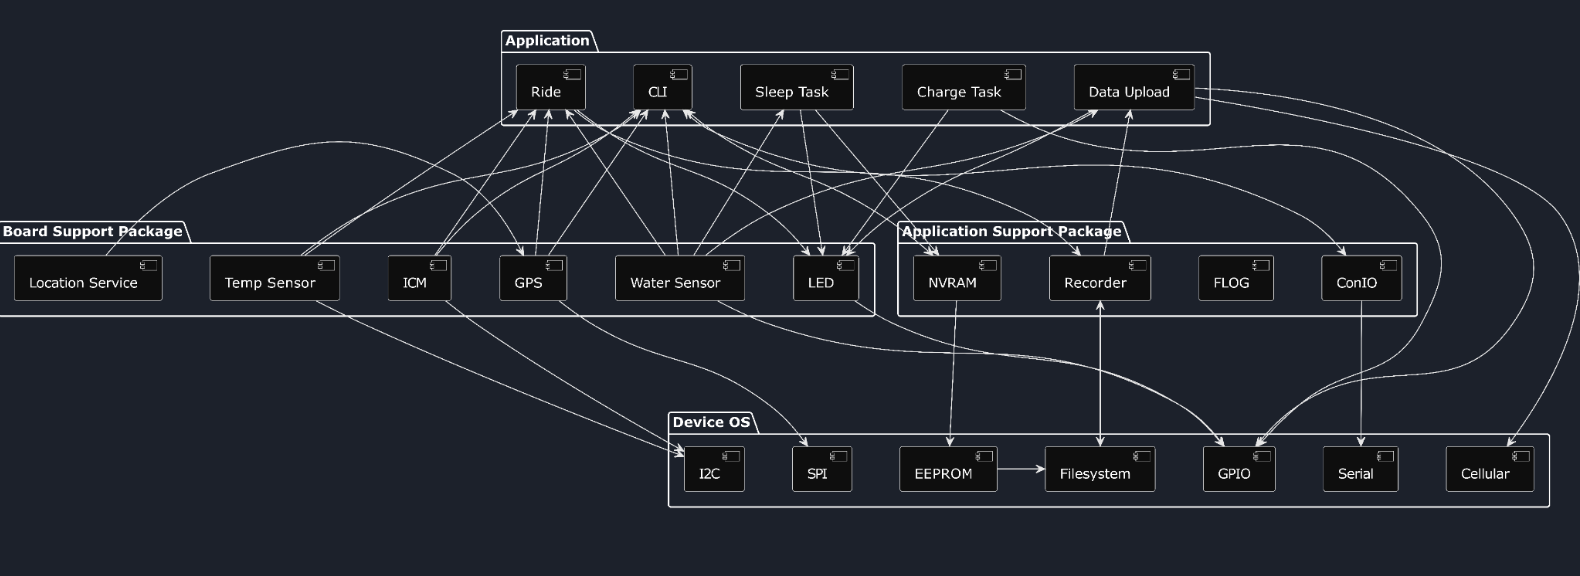
\includegraphics[height=1\textheight, width=1\textwidth, keepaspectratio]{images/sfSysArch.png}
\end{frame}

% To create a slide with a bullet list, use the following:
\begin{frame}{Hardware}
    \begin{itemize}
        \item Potting 
        \item Test and verify sensors
    \end{itemize}
    \centering    
    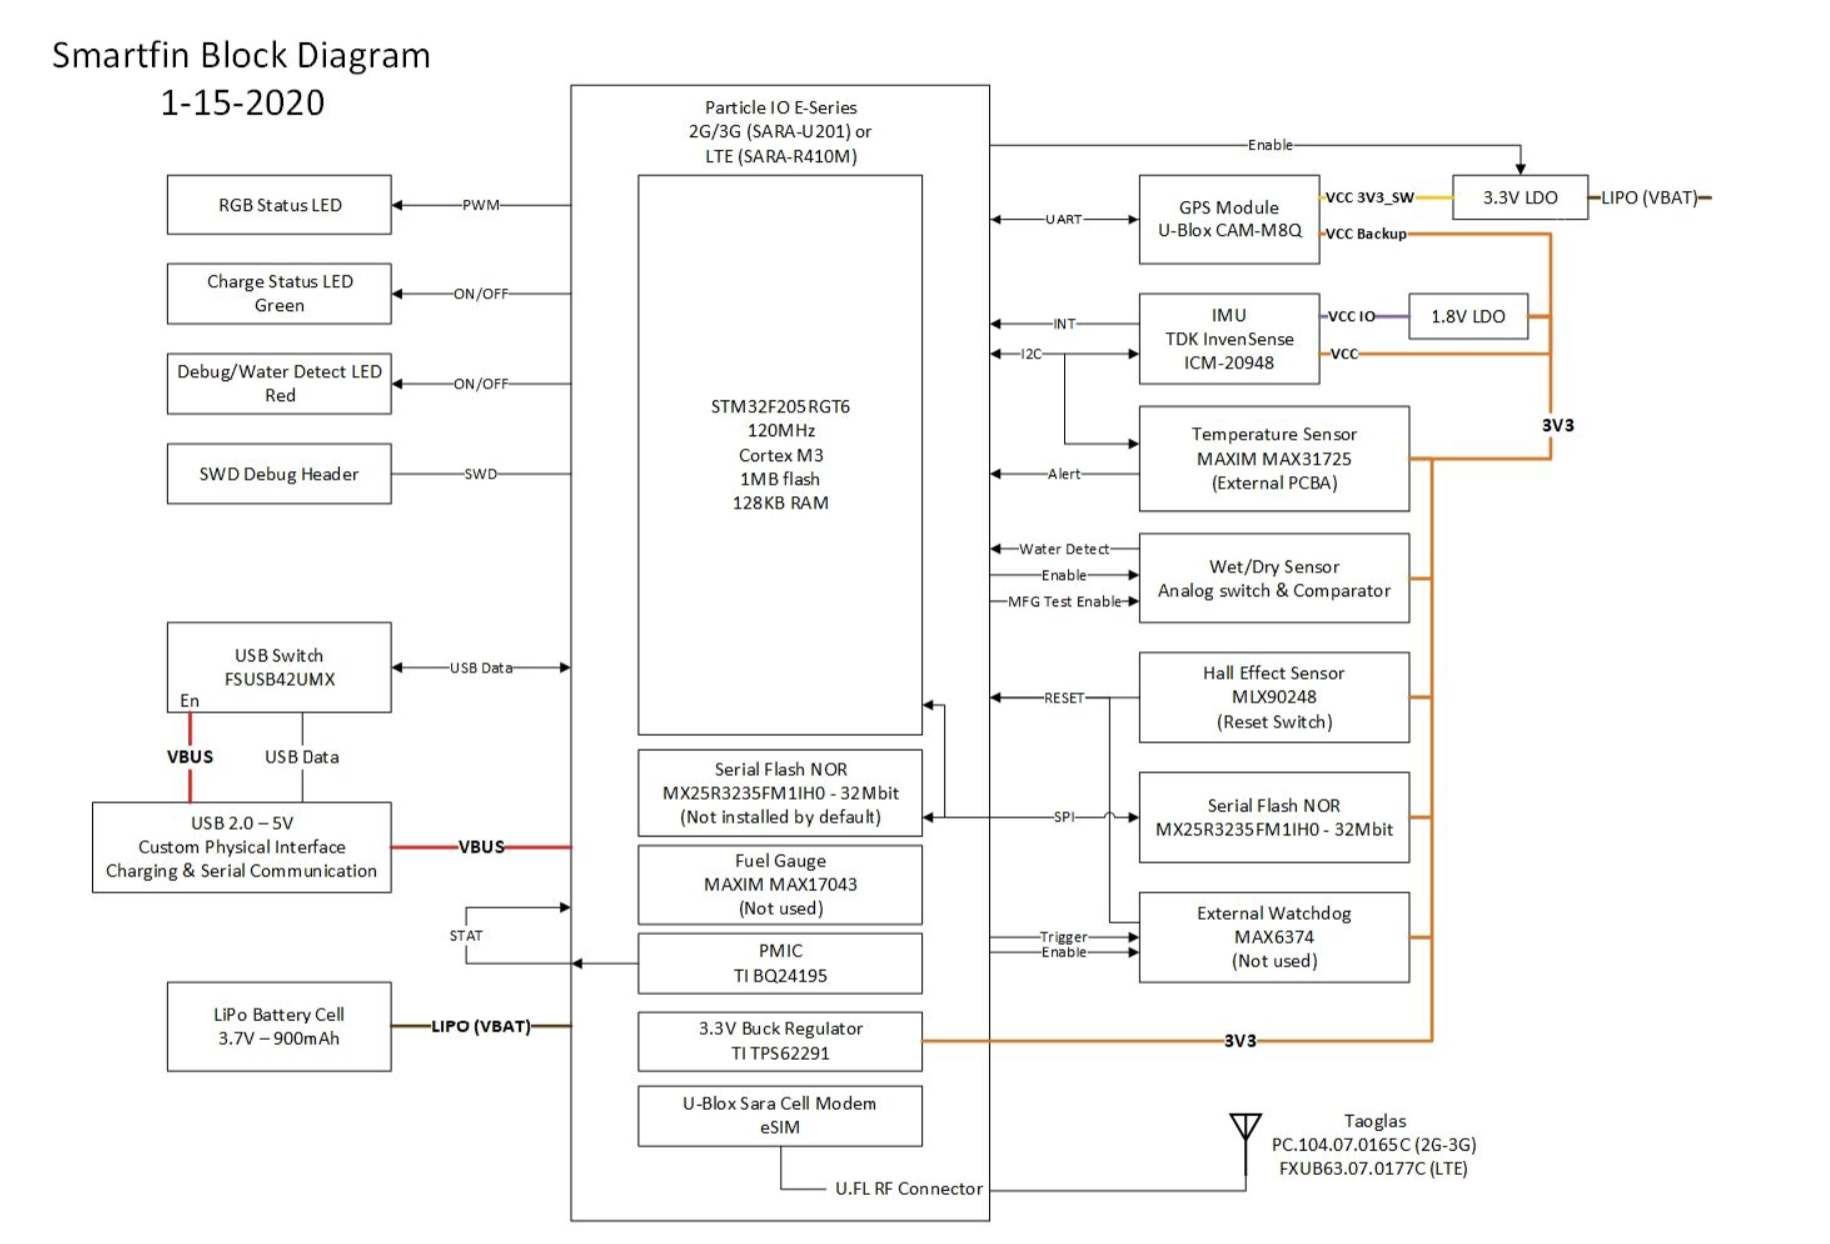
\includegraphics[height=0.6\textheight, width=0.6\textwidth, keepaspectratio]{images/schem.png}
\end{frame}

\begin{frame}{Software}
    \begin{itemize}
        \item Updating scheduler
        \begin{itemize} 
            \item FW2 $\rightarrow$ FW3
        \end{itemize}
        \item Calibration
    \end{itemize}    
\end{frame}

\begin{frame}{Improved Localization }
    \begin{itemize}
        \item IMU Accelerator
        \item Improved GPS tracking
    \end{itemize}   
    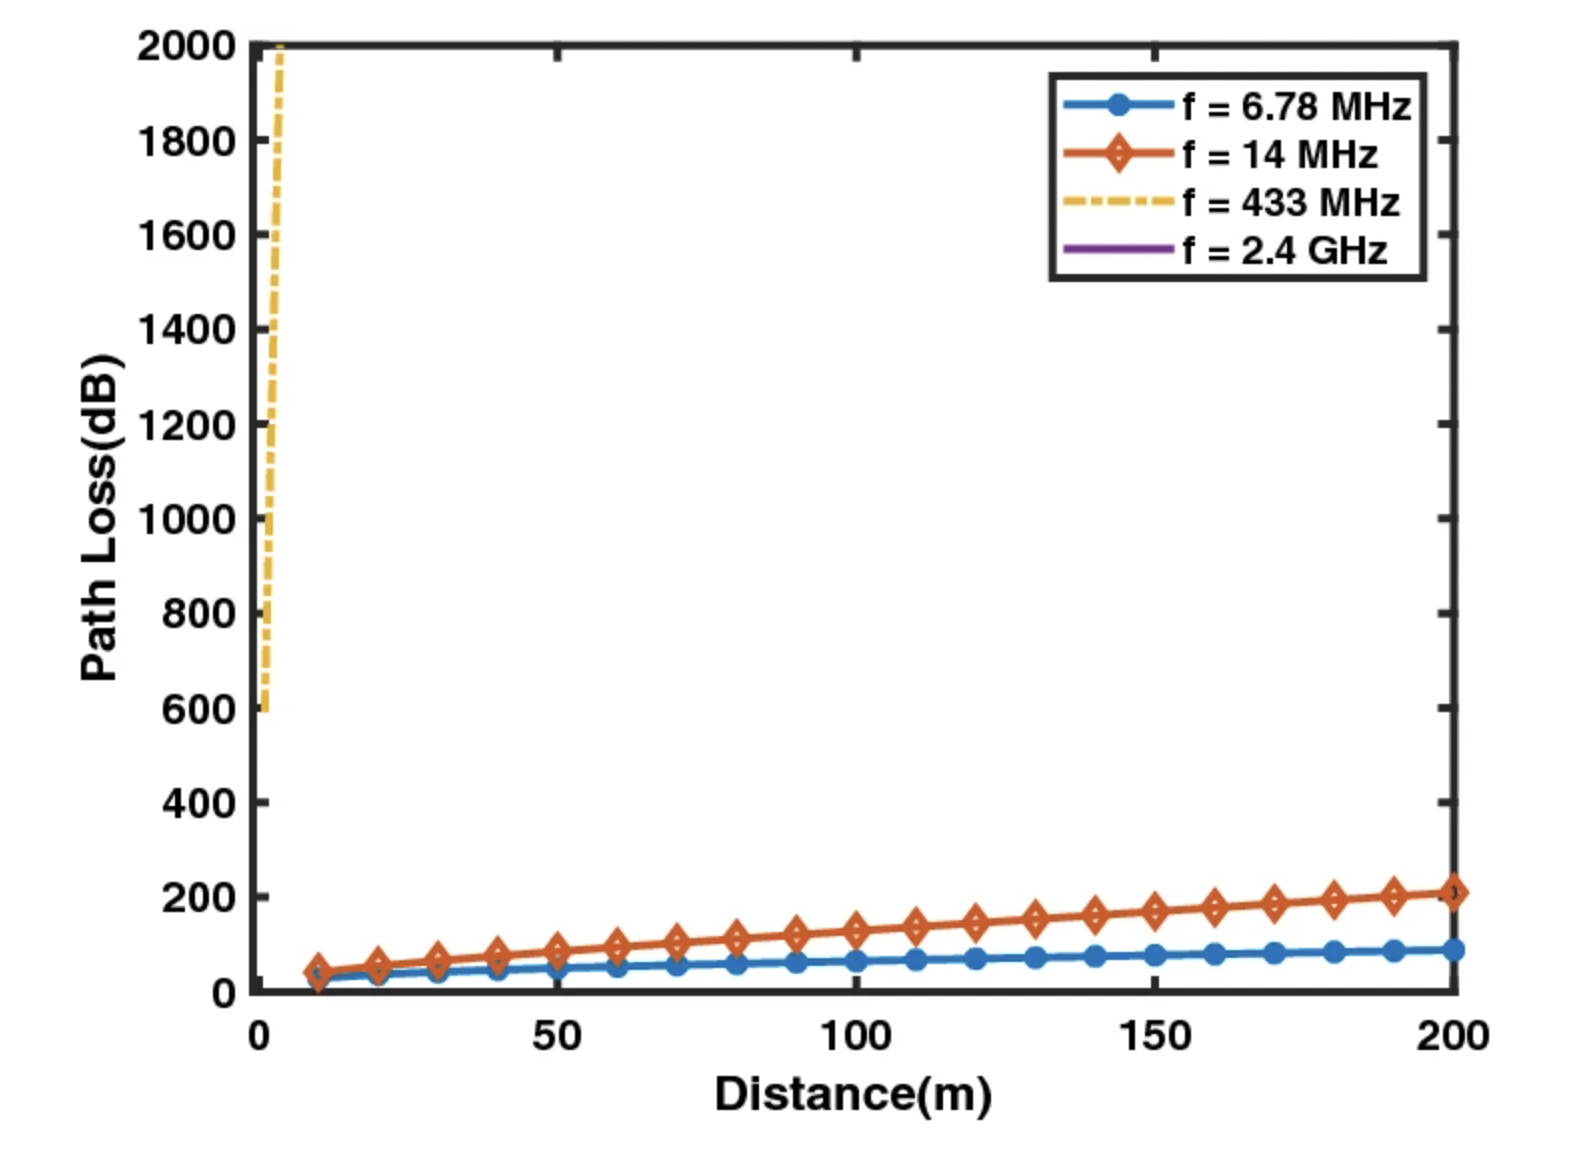
\includegraphics[height=0.6\textheight, width=0.6\textwidth, keepaspectratio]{images/path-loss.png}
    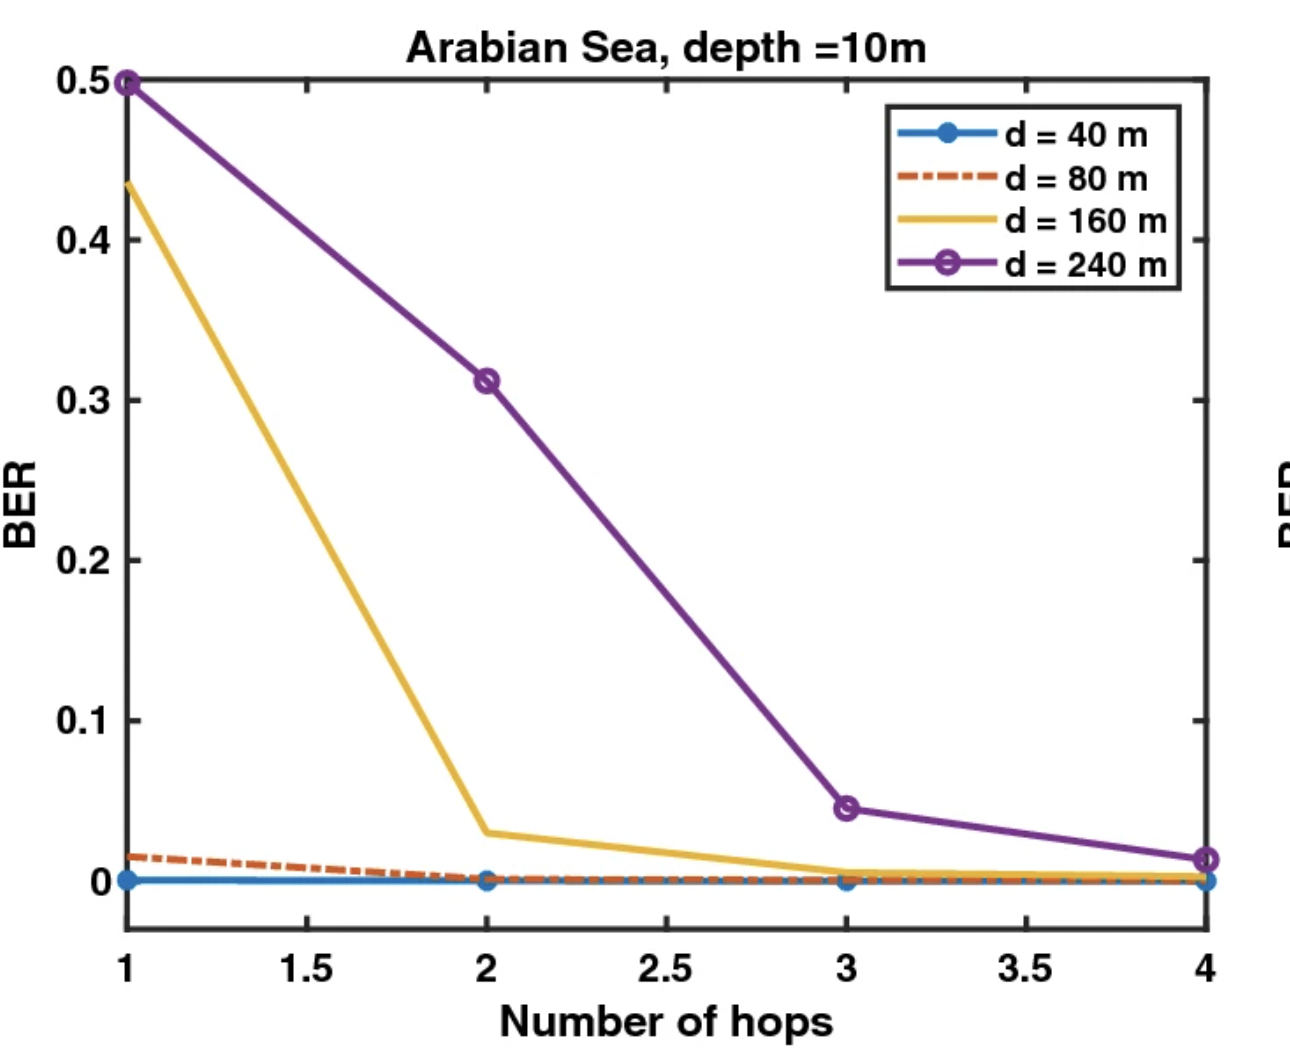
\includegraphics[height=0.6\textheight, width=0.6\textwidth, keepaspectratio]{images/multihop-biterror.png}
\end{frame}

% To create a slide with numbered list, use the following:
% \begin{frame}{TITLE}
%     \begin{enumerate}
%         \item ITEM 1
%         \item ITEM 2
%     \end{enumerate}
% \end{frame}

% To create a slide with a graphic:
% 1. Add the graphic to this folder (named picture.png)
% 2. Use the following:
% \begin{frame}{TITLE}
%     \centering
%     \includegraphics[height=0.7\textheight,width=0.7\textwidth,keepaspectratio]{picture.png}
% \end{frame}

% To create a slide with two columns, use the following:
% \begin{frame}{TITLE}
%     \begin{columns}
%         \begin{column}{0.5\textwidth}
%             COLUMN 1 BODY
%         \end{column}
%         \begin{column}{0.5\textwidth}
%             COLUMN 2 BODY
%         \end{column}
%     \end{columns}
% \end{frame}
